\title{ Determine Paths in the Same Homotopy Class }
\author{
        Yinan Zhang\\
        Department of Computer Science\\
        Dartmouth College\\
        Hanover, New Hampshire 03755, US
        \and
        Devin Balkcom \\
        Department of Computer Science\\
        Dartmouth College\\
        Hanover, New Hampshire 03755, US
}
\date{\today}

\documentclass[11pt]{article}
\usepackage{amsmath}
\usepackage{amsfonts}
\usepackage{graphicx}
\DeclareGraphicsExtensions{.pdf,.png,.jpg, .gif}
\usepackage{algpseudocode}

\newtheorem{theorem}{Theorem}[section]
\newtheorem{lemma}[theorem]{Lemma}
\newtheorem{definition}[theorem]{Definition}


\begin{document}
\maketitle

\begin{abstract}
Describing the  \ldots
\end{abstract}

\section{Introduction}
This is time for all good men to come to the aid of their party!

%%%%%%%%%%%%%%%%%%%%%%%%%%%%%%%%%%%%%%%%%%%%%%%%%%%%%%%%%%%%%%%%
%	Introducing Related Work
%
%%%%%%%%%%%%%%%%%%%%%%%%%%%%%%%%%%%%%%%%%%%%%%%%%%%%%%%%%%%%%%%%

\section{Related Work}\label{related work}

\indent\indent In this section, we first discuss the basics of sampling-based motion planning and the method of sampling on medial axis. With the information of positions and their clearance in c-space, we have samples as spheres. We then discuss the dual shapes of the union of balls which plays an important role in understanding the shape of c-space and its topology. Some works on graph theory and topology will finally be introduced.

%====================================
% Sampling Based Motion Planning
%====================================

\paragraph{A} \emph{Sampling-based Motion Planning} \hfill \\
\indent A robot is a movable object whose state can be described by $n$ parameters, or \emph{degrees of freedom} ($DOFs$). A point $<x_1, x_2, ..., x_n>$ in a n-dimensional space uniquely defines the configuration of a robot. Such space is called \emph{"Configuration Space"} or \emph{"C-space"}  ($C$). The subset of all feasible configurations is called the \emph{free space} (\emph{$C_{free}$}), while $C_{obst} = C \setminus C_{free}$ is the union of all infeasible configurations. \cite{UMAPRM} Path planning will generally be viewed as a search in a metric space $X$ for a continuous path from an initial state $x_{init}$ to a goal region $X_{goal} \subset X$. For a standard problem, $X = C$. \cite{RRT} What needs to be pointed out is that \emph{C-space} is very different from workspace which is usually formed by polygons. The shape of \emph{C-space} is usually unknown to us, unless the robot is a point. 

\indent Sampling-based algorithms have been very successful and have seen many applications in industry for planning in high dimension space. Probablistic Roadmap \cite{PRM} and Rapidly-Exploring Random Tree \cite{RRT} are two outstanding methods. The basic idea under these methods is to randomly sample feasible configurations in \emph{C-space} and connect nearby valid samples as edges to construct a graph or tree structure, which careless about the dimension problem. By connecting start and goal configurations to the roadmap, a graph search, e.g., A*, can be performed to extract a near optimal solution path.

\indent One disadvantage of these methods is that we can't study the topological structure of C-space using only the data structures constructed.

%====================================
% Sampling on medial axis
%====================================
\paragraph{B} \emph{Medial Axis Sampling} \hfill \\
\indent A simpler method that maintains the topology of \emph{C-space} but doesn't cover near optimal path is medial axis sampling. Medial Axis is also called Generallized Voronoi Diagram. The medial axis $MA(F)$ of free space $F$ is a strong deformation retract of $F$, which means $F$ can be continuously deformed onto $MA(F)$ while maintaining its topological structure. However, medial axis is hard to compute explicitly.

\indent In Figure \cite{Book}, sec. 5.6.3, Steven LaValle defined Medial Axis as "Let $(X, \rho)$ be a metric space. Let a \emph(maximal ball) be a ball $B(x,r) \subseteq X$ such that no other ball can be a proper subset the centers of all maximal balls trace out a one-dimensional set of points referred to as the \emph{medial axis}".  

\indent Mapping a pair of points $A$ and $B$ in free space onto $MA(F)$, there is a path between $A$ and $B$ if and only if there is a path between their images on $MA(F)$. Such path has a very nice property of the largest clearance from obstacles.

\indent Steven A. Wilmart \cite{MAPRM} sampled on the medial axis of free space to build up a probabilistic roadmap planner. He also showed that "it is possible to efficiently retract a configuration, free or otherwise, onto the medial axis of the free space without having to compute the medial axis explicitly".

\indent The basic idea of the algorithm proposed in \cite{MAPRM} is: given a point $A$ and its nearest point on the boundary of obstacles $A'$, a ray start from $A$ with direction $\overrightarrow{A'A}$ will always intersect with $MA(F)$.

\indent This method results in sampling more nodes in narrow corridors, which is beneficial for improving performance on problems requiring traversal of such corridors.

\indent However, such property makes the sampling method biased heavily towards certain portions of the medial axis. These biased property tend to ignore more critical parts of the space: large open free space. Sampling uniformly on the medial axis is sometimes more helpful.

\indent Hsin-Yi (Cindy) Yeh \cite{UMAPRM} solved this problem by putting some random "sticks" with random directions in free space. Any surfaces will intersect uniformly with these sticks, thus searching on sticks to find points that intersect with medial axis will give nodes uniformly distributed on the medial axis.

\indent Figure \ref{fig:Medial Axis} visualizes the shape of medial axis of a rectangle.

\begin{figure}
	\center{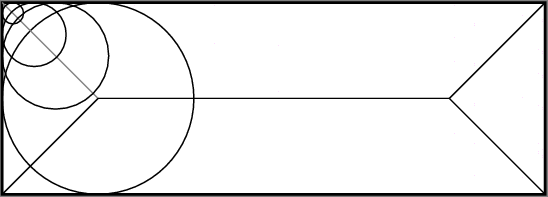
\includegraphics[scale=0.35]{./pics/MA.png}}
	\caption{\label{fig:Medial Axis} Sampling on the Medial Axis of a rectangle space.\cite{Book}}
\end{figure}

%====================================
% Dual shapes of unions of balls
%====================================

\paragraph{C} \emph{Dual Shapes of Unions of Balls} \hfill\\
\indent Approximating the shape of an unknown area to study its properties is a very commonly used method. We have seen many such ideas in the study of biogeometry. As for robotics, a few people began to notice the achievements from biogeometry study and tried to apply similar methods to study the shape of \emph{C-space}. 

\indent Zoe McCarthy \cite{PathNonexistance} used samples generated by PRM to form the $\alpha$-shape of \emph{C-space}. She then proved there doesn't exist a path between a pair of configurations by proving they are in two different disconnected components of the shape. She declared it was the first time $\alpha$-shape is being used in motion planning.

\indent Define a \emph{simplicial complex} $D$: a collection of simplices such that if $\bigtriangleup_T \subseteq D$ ( $\bigtriangleup_T$ is the convex hull of $T$ ), then if $U \subseteq T$, we have $\bigtriangleup_U \subseteq D$ and also that the intersection of two simplices in $D$ is either empty or another simplex in $D$. The $\alpha$-shape of a set of points $S$ is a generalization of the convex hull of those points. \cite{PathNonexistance}. H. Edelsbrunner first introduced them in \cite{PointSetShape}. By choosing different value of the one parameter $\alpha$, we can have a family of shapes with the same set of points. An example of $\alpha$-shape is in Figure \ref{fig:Alpha-shape}.

\indent Choosing the best $\alpha$ value could be a bothering work. Assuming weighted points in the point set, by using a generalization of the Delaunay Triangulation, the Regular Triangulation, we can construct another shape using weights as flexible $\alpha$'s. Points with weights can be considered as balls. H. Edelsbrunner gave us this idea in \cite{DualShape}. Such shapes are also called Dual Shapes or Dual complex of unions of balls. The weighted $\alpha$-shape captures the topology of the union of balls with different radii. Figure \ref{fig:Dual Shape} shows an example of such weighted $\alpha$-shape.

\begin{figure}
	\center{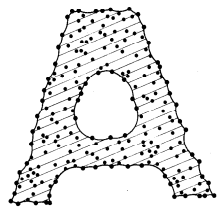
\includegraphics[scale=0.7]{./pics/alphaShape.png}}
	\caption{\label{fig:Alpha-shape} An example of $\alpha$-shape. \cite{PointSetShape}}
\end{figure}

\begin{figure}
	\center{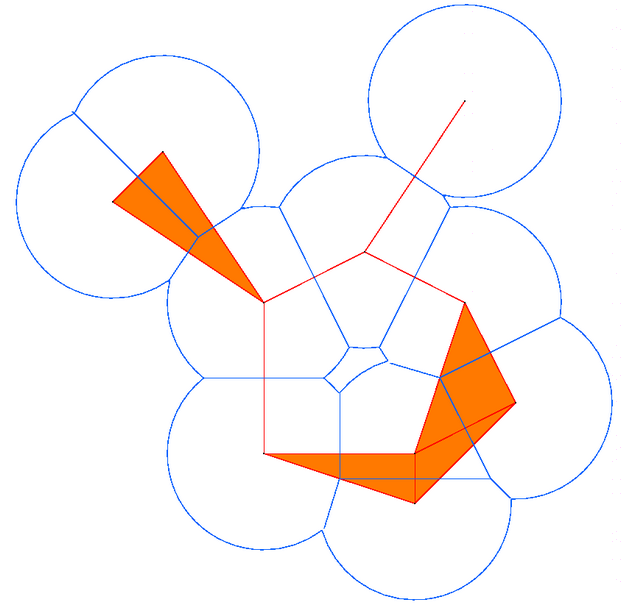
\includegraphics[scale=0.30]{./pics/dualshape.png}}
	\caption{\label{fig:Dual Shape} An example of weighted $\alpha$-shape for a union of balls. \cite{DualShape}}
\end{figure}

%====================================
% Betti Numbers
%====================================
\paragraph{D} \emph{Betti Numbers} \hfill \\
\indent In algebraic topology, the Betti Numbers are used to distinguish topological spaces based on the connectivity of n-dimensional simplicial complexes. Informally, the \emph{n-th} Betti number ($\beta_n$) represents the rank of the \emph{n-th} homology group, which tells us the maximum number of cuts that can be mad before diving a surface into two pieces. \cite{betti wiki}

\indent An example of Betti numbers will be a torus. Figure \ref{fig:Torus}

\indent H. Edelsbrunner introduced a way to compute $n-th$ Betti number in \cite{Edel Book}, where he uses gaussian ellimination to compute the betti numbers with adjacency matrix.

\indent Vanessa Robins \cite{alpha betti} provided more detailed explains and proofs on computing betti numbers. What's more, she put more thoughts on computing betti numbers for alpha shapes.

\begin{figure}
	\center{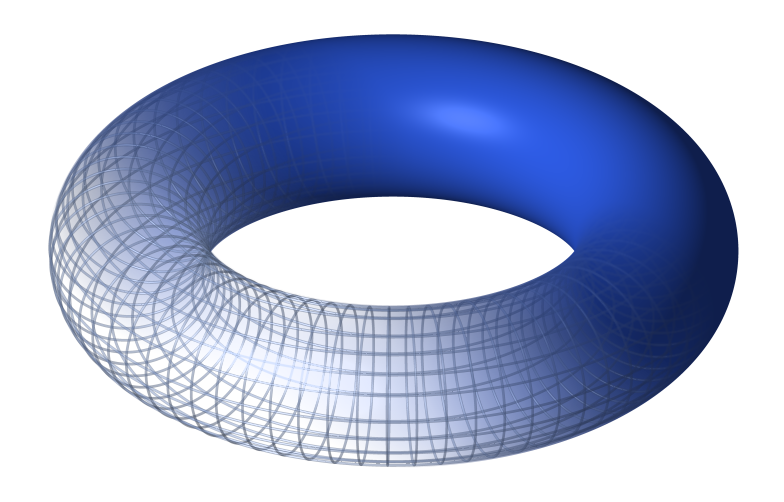
\includegraphics[scale=0.26]{./pics/Torus.png}}
	\caption{\label{fig:Torus} The torus has one connected component($\beta_0$), two circular holes ($\beta_1$,the one in the center and the one in the middle of the "donut"), and one two-dimensional void ($\beta_2$, the inside of the "donut").\cite{betti wiki}}
\end{figure}


%%%%%%%%%%%%%%%%%%%%%%%%%%%%%%%%%%%%%%%%%%%%%%%%%%%%%%%%%%%%%%%%
%	Introducing Our Algorithm
%
%%%%%%%%%%%%%%%%%%%%%%%%%%%%%%%%%%%%%%%%%%%%%%%%%%%%%%%%%%%%%%%%

\section{Our Method}\label{method}

\indent \indent Traditionally, sampling based algorithms will build a graph for configuration space. These kind of graphs are proved to be able to find near optimal path, but can hardly be used to analysis the topology of paths. We want to to build a stronger representation of c-space that is both able to cover optimal path and study the topological structure of c-space. In this section, we are trying to solve the problem in 2D and answer the question "Is two paths in the same homotopy class" as a start point of using our method to study the topology of \emph{C-space}. We will first give the outline of the algorithm, and explain each step in detail. 

\paragraph{A} \emph{The Algorithm outline} \hfill \\
\indent Before starting introducing our algorithm, we firstly clarify some preliminary tools we can have: 

%%%%%%%%%%%%%%%%================================================>>>>>>>>>>>>>>>>>>>>>>>>>>>>>>
%%%%%%  We need to name our algorithm
%%%%%%  Seriously
%---------------------------------------------------------------------------------------------
\begin{figure}
  \begin{algorithmic}[1]
  \Function{OurAlgorithm}{\emph{C-space}}
    \State $pntset \gets$ randomly generated points in free space.
    \State $maSamples \gets$ Empty Set.
    \State $l \gets $ stick length.	 
	\For{$point \in pntset$}
		\State $dir \gets$ random direction  
		\State $stick \gets$ ( point, l, dir ) \Comment{start point+length+direction=a stick}
		\If{ $stick$ intersects with the medial axis }
		
			\indent\indent $sample \gets$ stick.search()
			
			\indent\indent $radius \gets$ clearance( sample ) \Comment{get the clearance at this point}
			
			\indent\indent $maSamples.append( ball(sample, radius) )$
		\EndIf
	\EndFor
	
	\Return $maSamples$;
  \EndFunction
  \end{algorithmic}
  \caption{Algorithm Outline}
\end{figure}

\paragraph{B} \emph{Sampling in C-space} \hfill \\

\paragraph{C} \emph{Constructing Topology Roadmap of C-space} \hfill \\

\paragraph{D} \emph{Breaking A Graph into Loop-free Parts} \hfill\\

\paragraph{E} \emph{Determine Paths Homotopy Class} \hfill \\


\section{Good Properties}\label{properties}

\section{Experiments}\label{experiments}
We now describe the some experiments and their results.

\section{Conclusions and Future Work}\label{conclusions}
We worked hard, and achieved very little.

\bibliographystyle{abbrv}
\begin{thebibliography}{1}

  \bibitem{Book} Steven M. LaValle, "Planning Algorithms", Cambridge University Press, ISBN 0-521-86205-1, 2006.
  \bibitem{UMAPRM} Yeh, Hsin-Yi Cindy, et al. "UMAPRM: Uniformly Sampling the Medial Axis."
  \bibitem{RRT} LaValle, Steven M. "Rapidly-Exploring Random Trees A New Tool for Path Planning." (1998).
  \bibitem{PRM} L. E. Kavraki, P. Svestka, L. E. K. P. Vestka, J. claude Latombe, and M. H. Overmars, “Probabilistic roadmaps for path planning in high-dimensional configuration spaces,” IEEE Trans. Robot. Autom., vol. 12, pp. 566–580, 1996.
  \bibitem{MAPRM} Wilmarth, Steven A., Nancy M. Amato, and Peter F. Stiller. "MAPRM: A probabilistic roadmap planner with sampling on the medial axis of the free space." Robotics and Automation, 1999. Proceedings. 1999 IEEE International Conference on. Vol. 2. IEEE, 1999.
  \bibitem{DualShape} Edelsbrunner, Herbert. "The union of balls and its dual shape." Proceedings of the ninth annual symposium on Computational geometry. ACM, 1993.
  \bibitem{PointSetShape} Edelsbrunner, Herbert; Kirkpatrick, David G.; Seidel, Raimund (1983), "On the shape of a set of points in the plane", IEEE Transactions on Information Theory 29 (4): 551–559, doi:10.1109/TIT.1983.1056714.
  \bibitem{PathNonexistance} Z. McCarthy. Bretl, and S. Hutchinson, "Proving path non-existence using sampling and alpha shapes," in IEEE International Conference on Robotics and Automation (ICRA), May 2012.
  \bibitem{betti wiki} "Betti Number", From Wikipedia -- The Free Encyclopedia. ( $http://en.wikipedia.org/wiki/Betti_number$ )    
  \bibitem{Edel Book}Edelsbrunner, Herbert, and John Harer. "Computational topology: an introduction." American Mathematical Soc., 2010. page. 88 - 93.
  \bibitem{alpha betti} Robins, Vanessa. "Computational topology for point data: Betti numbers of α-shapes." Morphology of Condensed Matter. Springer Berlin Heidelberg, 2002. 261-274.
\end{thebibliography}

\end{document}